\section{ANALISIS E INTERPRETACION DE RESULTADOS} 


\subsection{Parte 1: Actividades Encargadas}
	\begin{itemize}
		\item ¿Con qué comando(s) exportaría la imagen de Docker de Microsoft SQL Server a otra PC o servidor?
                      \begin{figure}[H]
		\begin{center}
		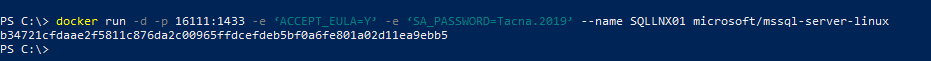
\includegraphics[width=15cm]{./Imagenes/6}
		\end{center}
		\end{figure} 
		\item ¿Con qué comando(s) podría generar dos volúmenes para un contenedor para distribuir en un volumen el Archivo de Datos (.mdf) y en otro el Archivo Log (.ldf)? 
                     \begin{figure}[H]
		\begin{center}
		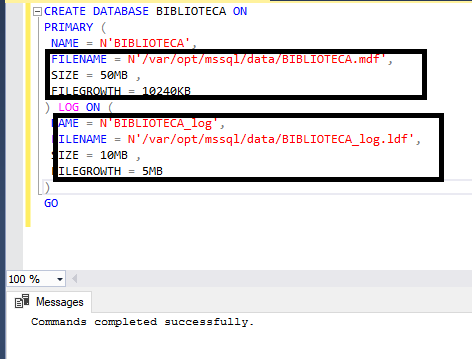
\includegraphics[width=7cm]{./Imagenes/18}
		\end{center}
		\end{figure} 
		\item Genere un nuevo contenedor y cree la base de datos con las siguientes características.
                      \begin{figure}[H]
		\begin{center}
		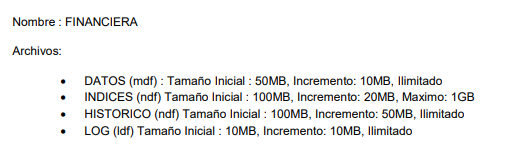
\includegraphics[width=7cm]{./Imagenes/30}
		\end{center}
		\end{figure} 
		\item  ¿Cuál sería el script SQL que generaría esta base de datos?
\begin{figure}[H]
		\begin{center}
		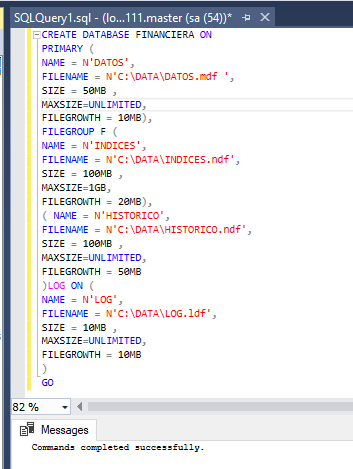
\includegraphics[width=10cm]{./Imagenes/t4}
		\end{center}
		\end{figure}
	\end{itemize}



